\chapter{N-subjettiness\label{sec:nsubj}}

Highly boosted particles can result from the decay of high-mass resonances, whose production in the LHC is made possible by the high collision energies achievable. The decay products of a boosted object appear as a collimated spray of tracks in the detector; with a sufficiently high boost factor and thus sufficiently high collimation, these decay products can be reconstructed as a single jet and are thus not identified as distinct objects. Techniques for probing jet substructure are important for identifying and analyzing boosted jets. One method is the use of N-subjettiness ($\tau_{N}$), a parameter that measures the degree to which the energy within a jet is aligned along N candidate subjet axes\newline
The formula for N-subjettiness is as follows:

\begin{equation}
\tau_{N} = \cfrac{1}{d_{0}}\sum_{k}^{}p_{T,k}min(\Delta R_{1,k},\Delta R_{2,k},\dots,\Delta R_{N,k})
\label{eq:Nsubj}
\end{equation}

\noindent The index \emph{k} goes over all the constituent particles in the jet, $p_{T,k}$ is the transverse momentum of the $k^{th}$ particle, and $\Delta$R$_{n,k}$ is the distance in $\eta-\phi$ space between the $k^{th}$ particle and the axis of the $n^{th}$ candidate subjet. The term $d_{0}$ is given by

\begin{equation}
d_{0} = \sum_{k}^{}p_{T,k}R_0
\label{eq:d0}
\end{equation}

\noindent where $R_{0}$ is the radius used in the original jet clustering algorithm \cite{Thaler:2010tr}.\newline
In a jet whose particles are closely aligned with N or fewer subjets, the terms $p_{T,k}$min($\Delta$R$_{1,k}$, $\Delta$R$_{2,k}$, \dots, $\Delta$R$_{N,k}$) in the sum will be very small, and thus $\tau_{N}$ will be closer to zero, while in a jet whose energy is distributed away from the N subjet axes will have a larger value of $\tau_{N}$ and must have at least N + 1 subjets.\newline
N-subjettiness has been used successfully in the identification of boosted objects such as top quarks and $W$ bosons. A new use of N-subjettiness for identifying jets seeded by boosted tau pairs (referred to as boosted ditau jets) was probed in a theoretical study by Englert et al. \cite{Englert:2011iz}, which suggested that the ratio $\tau_{3}$/$\tau_{1}$ could provide discrimination between boosted ditau jets and QCD jets. This study used 14-TeV Monte Carlo signal and background samples under conditions of zero pileup, where the signal process was  $h_{1}\rightarrow 2a_{1}\rightarrow 4\tau$, with all inclusive tau decay modes considered.\newline
In this study, N-subjettiness ratios $\tau_{3}/\tau_{1}$, $\tau_{2}/\tau_{1}$, $\tau_{1}/\tau_{2}$, $\tau_{2}/\tau_{3}$, and $\tau_{3}/\tau_{4}$  were explored for their possible discriminatory power. An important issue that arose was the influence of pileup on the N-subjettiness distribution, which tends to impair the discriminatory power of N-subjettiness ratios for the signal; for instance, the mean of the $\tau_{3}/\tau_{1}$ distribution was observed to increase with increasing pileup for signal Monte Carlo, causing it to become increasingly indistinguishable from the $\tau_{3}/\tau_{1}$ distribution for jets from $W$+NJets events. Jet pruning was used to remove pileup from jets, and although this recovered some of the discriminatory power when comparing unit-normalized signal and $W$+NJets Monte Carlo $\tau_{3}/\tau_{1}$ distribution shapes, further analysis -- comparing signal Monte Carlo and all other background Monte Carlo samples except QCD, after applying pileup reweighting and all the preselection cuts to these events -- has not shown significant discrimination between signal and background. Also, as a result of the jet pruning, significant number of jets were left with only 3 or fewer constituents, resulting in $\tau_{3}/\tau_{1}$ values of exactly 0. This suggests that less aggressive methods of pileup removal from jets should be explored. Figures~\ref{fig:nsubjettiness-ratios-lowMT} and~\ref{fig:nsubjettiness-ratios-highMT} show the distributions of two N-subjettiness ratios, $\tau_{3}/\tau_{1}$ and $\tau_{1}/\tau_{2}$, for the low and high $M_{T}$ bins, illustrating both the currently insufficient discriminatory power of these variables and the problematic peak at zero (for $\tau_{3}/\tau_{1}$) caused by jet pruning. More investigation will eventually be required to find a more effective method of pileup removal and potentially an improvement in discriminatory power for N-subjettiness ratios.

\begin{figure}[hbtp]
  \begin{center}
    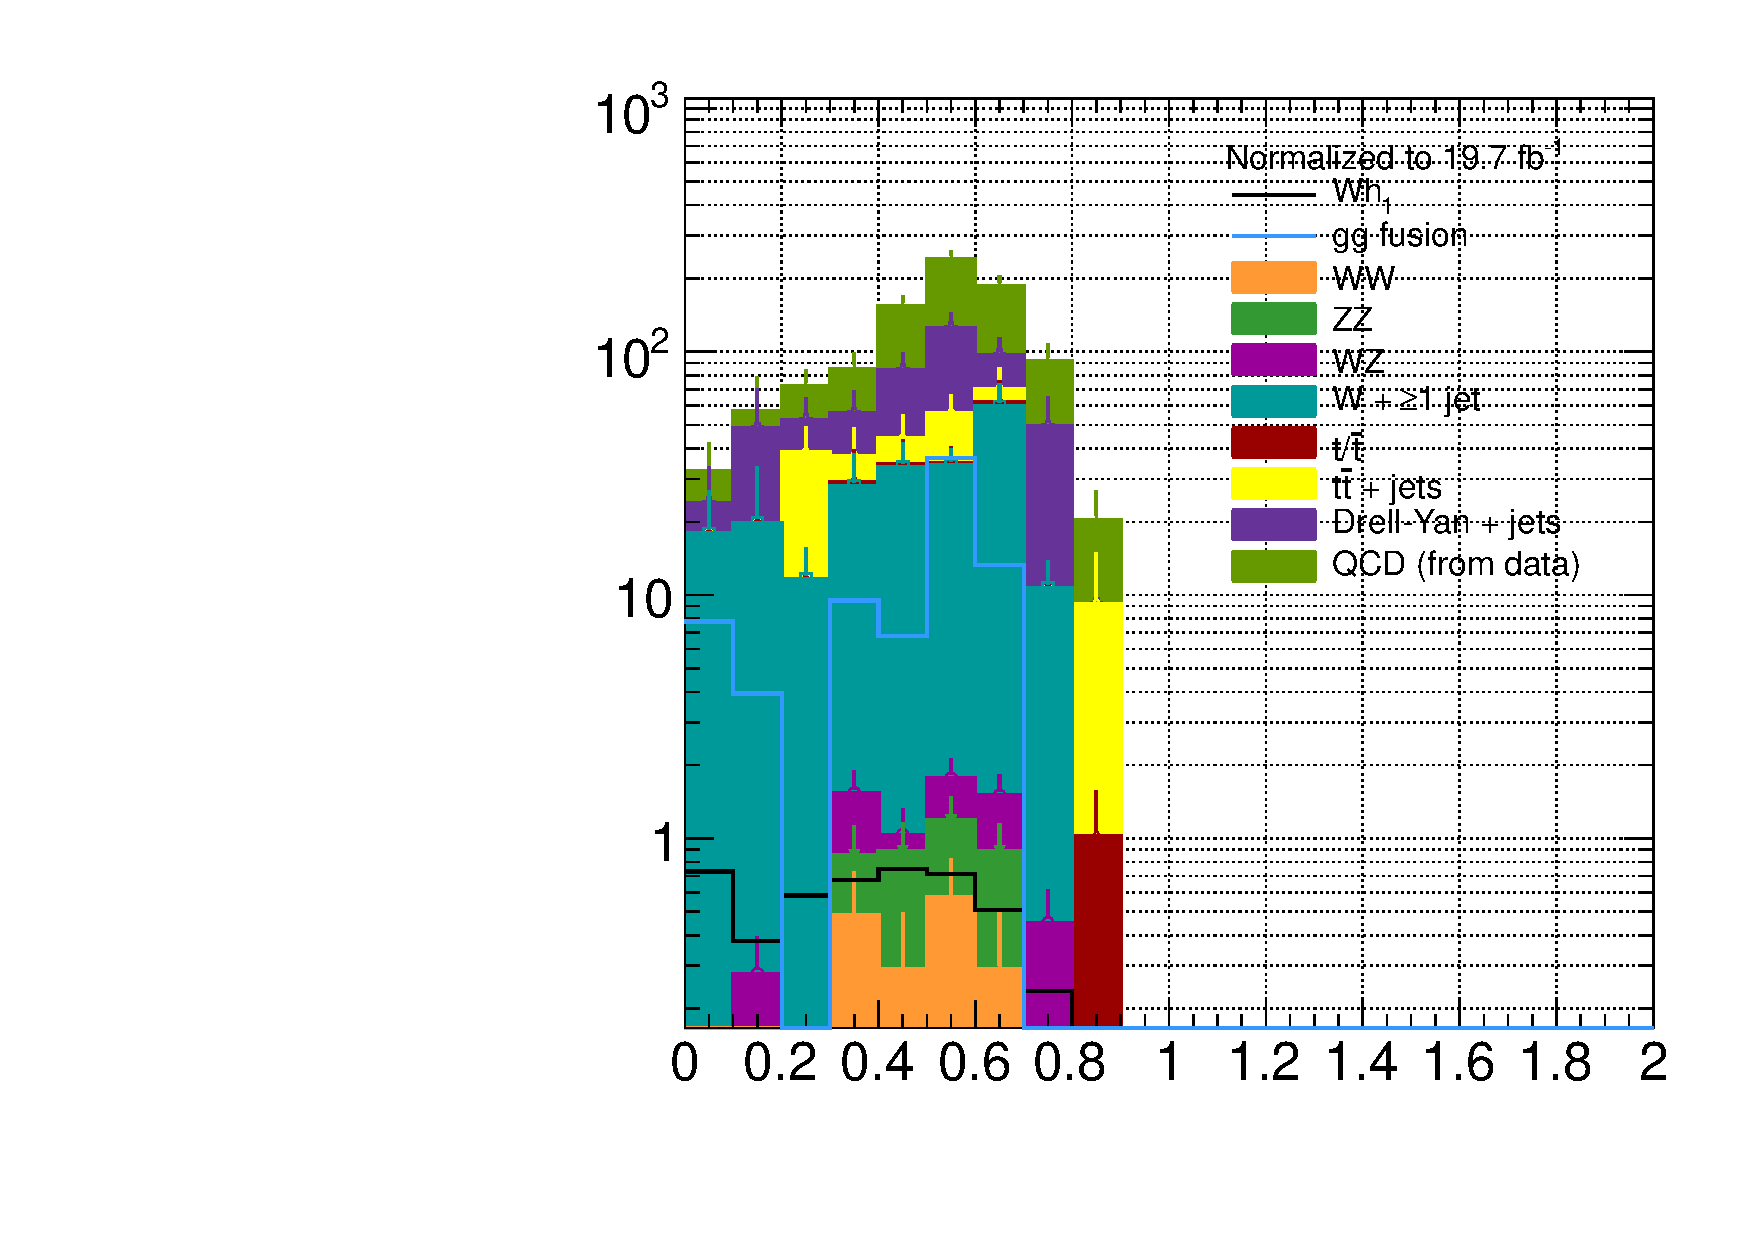
\includegraphics[width=1.2\cmsFigWidth]{figures/sigVsBkg_t3t1_lowMT}
    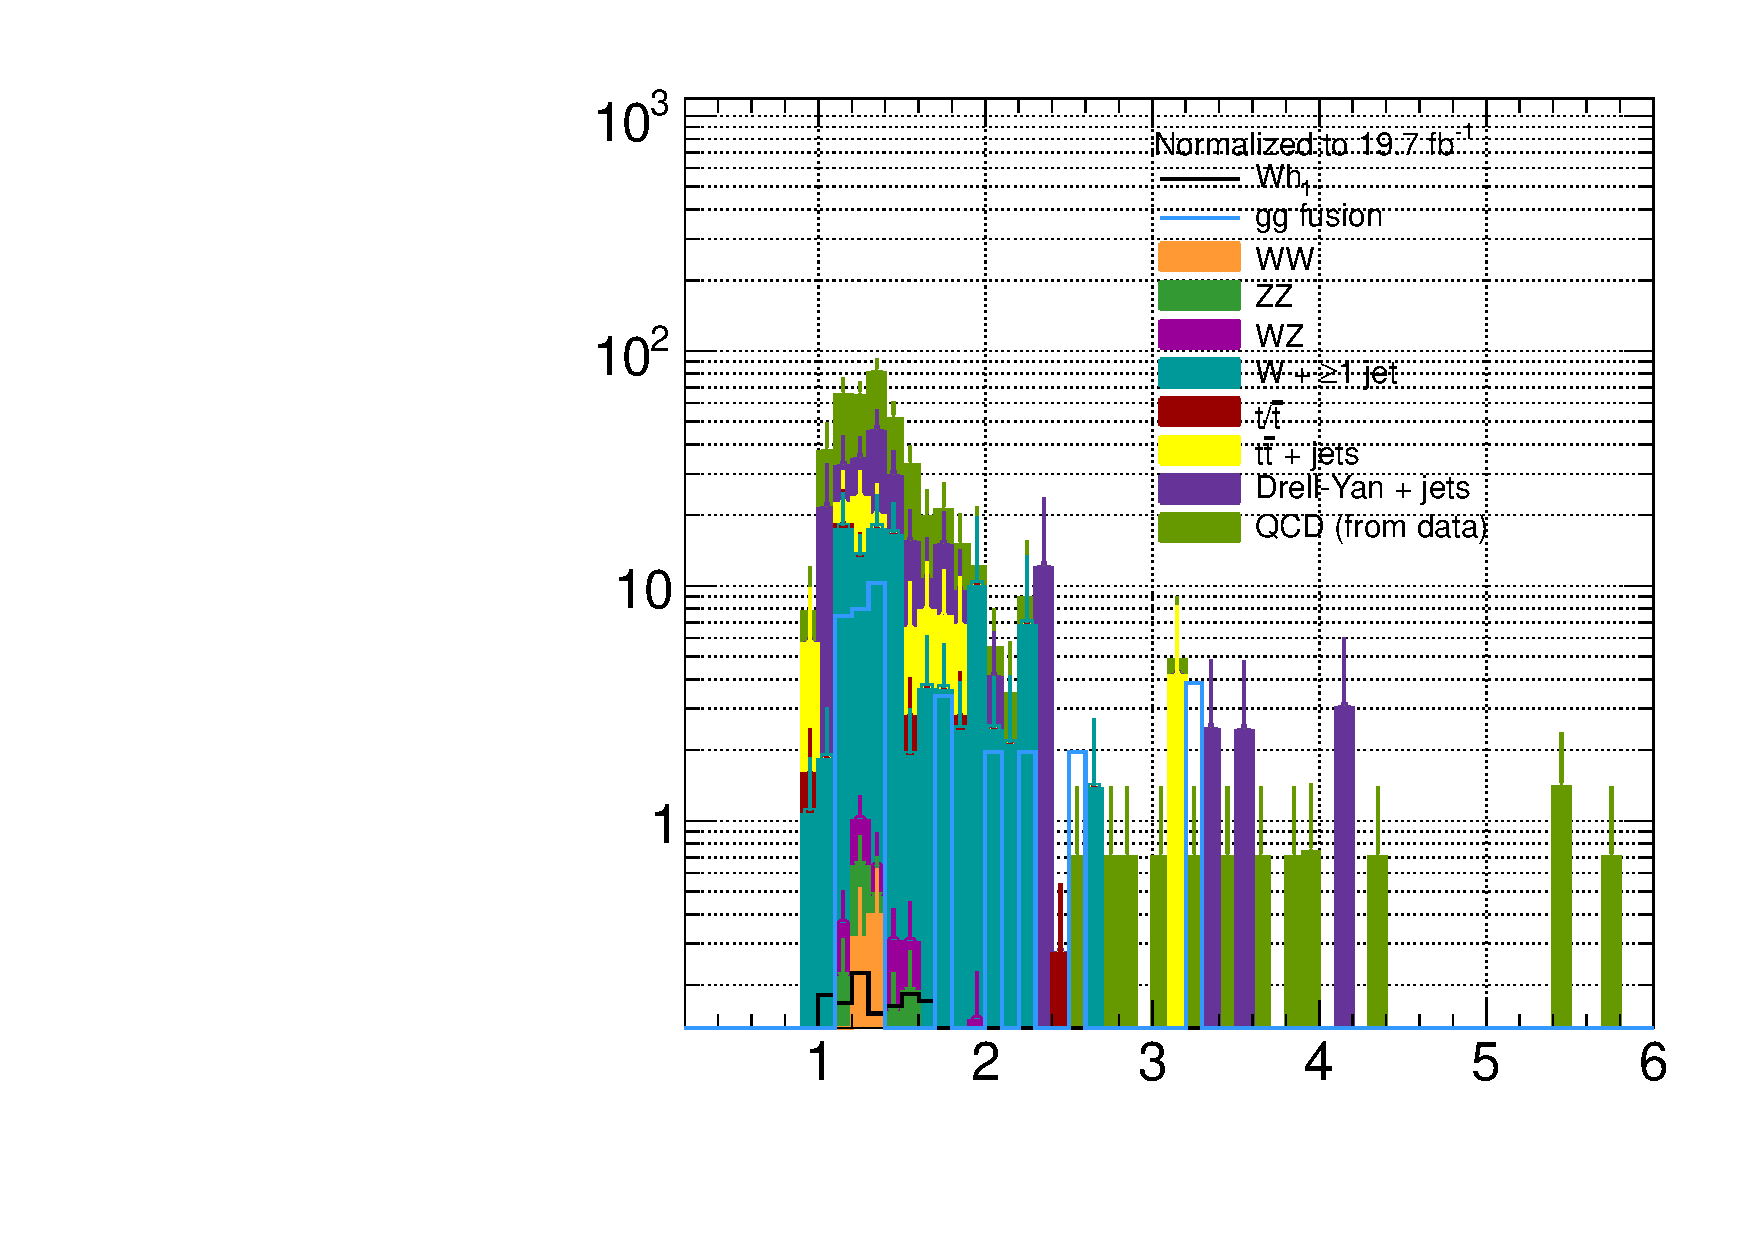
\includegraphics[width=1.2\cmsFigWidth]{figures/sigVsBkg_t1t2_lowMT}
    \caption{Examples of N-subjettiness ratio distributions for the low-$M_{T}$ bin, comparing distributions for two signal models and all backgrounds discussed in Sec.~\ref{sec:evtsel} including data-driven QCD, after all the preselection cuts have been applied. (\cmsLeft) $\tau_{3}/\tau_{1}$. (\cmsRight) $\tau_{1}/\tau_{2}$.}
    \label{fig:nsubjettiness-ratios-lowMT}
  \end{center}
\end{figure}

\begin{figure}[hbtp]
  \begin{center}
    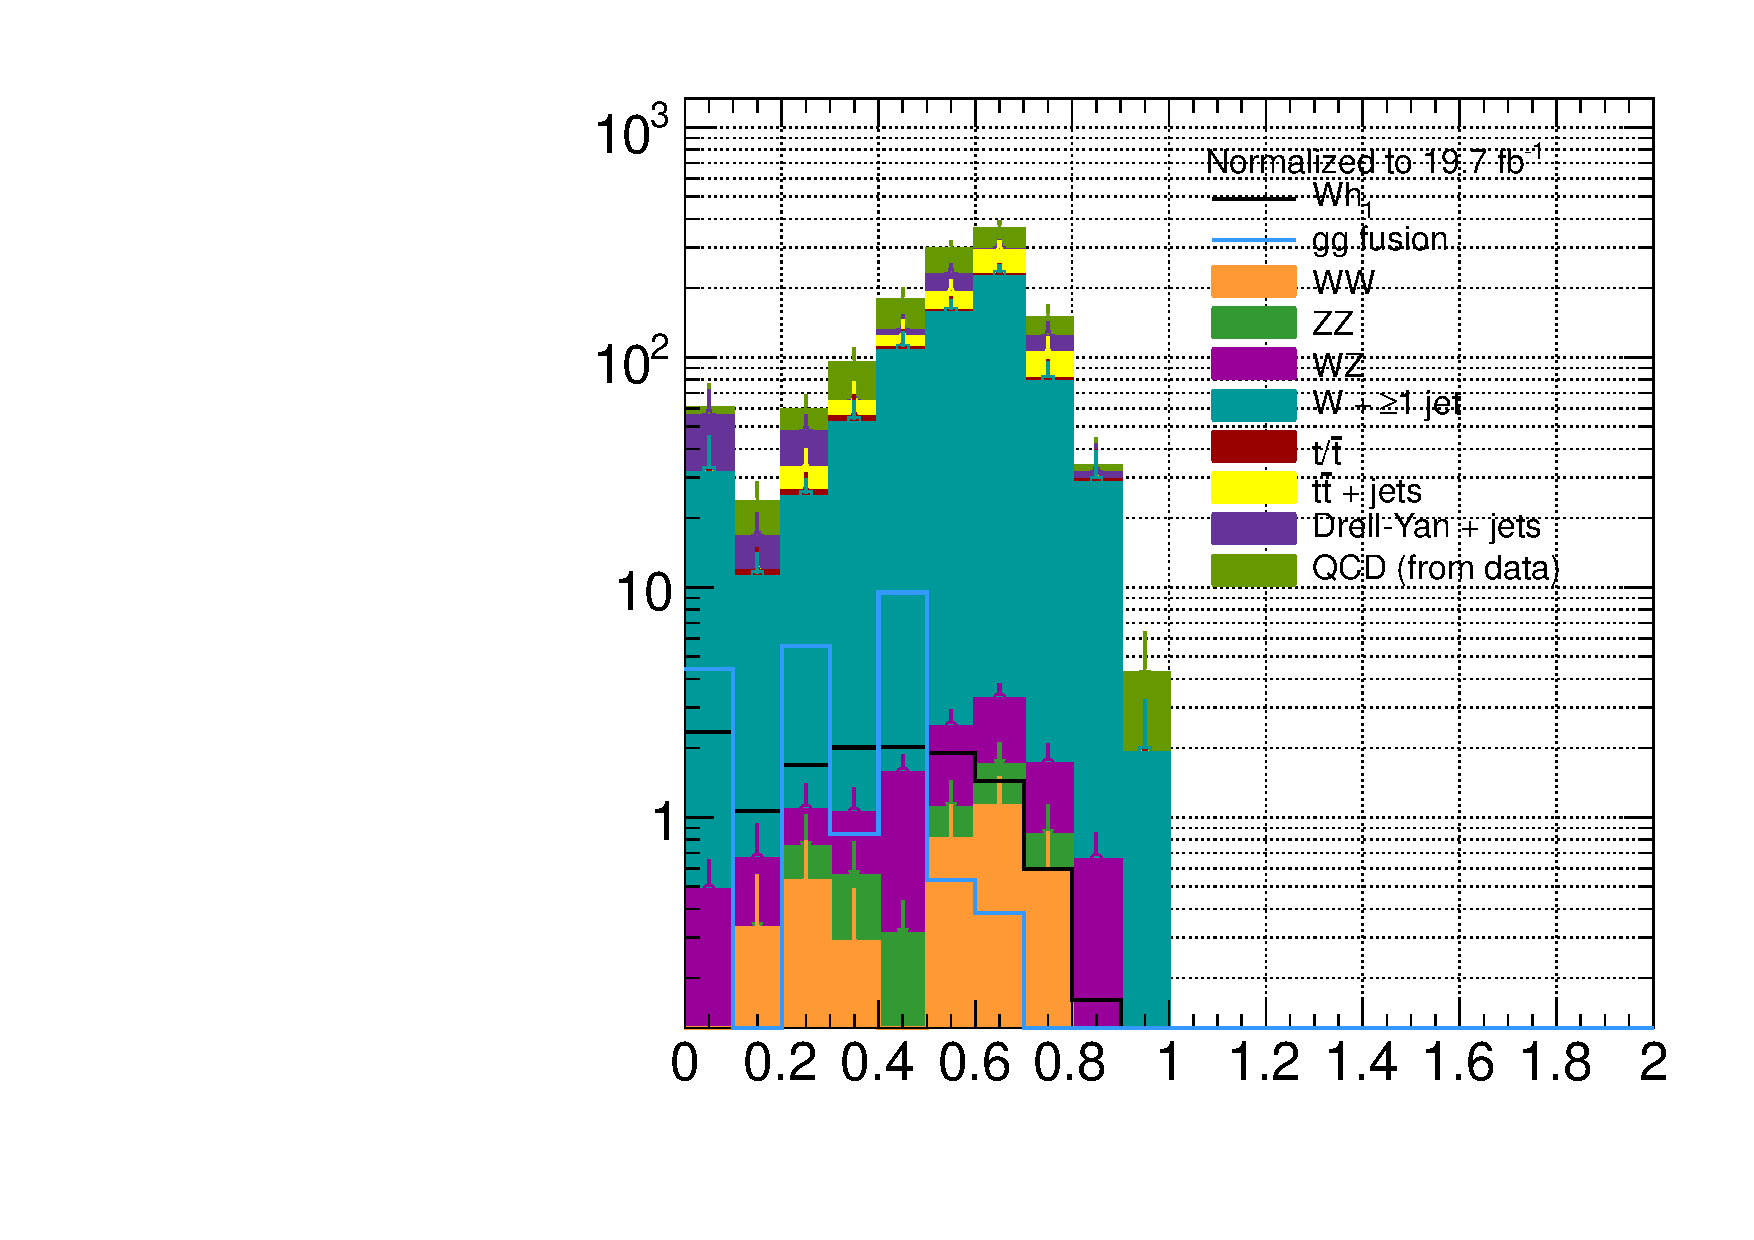
\includegraphics[width=1.2\cmsFigWidth]{figures/sigVsBkg_t3t1_highMT}
    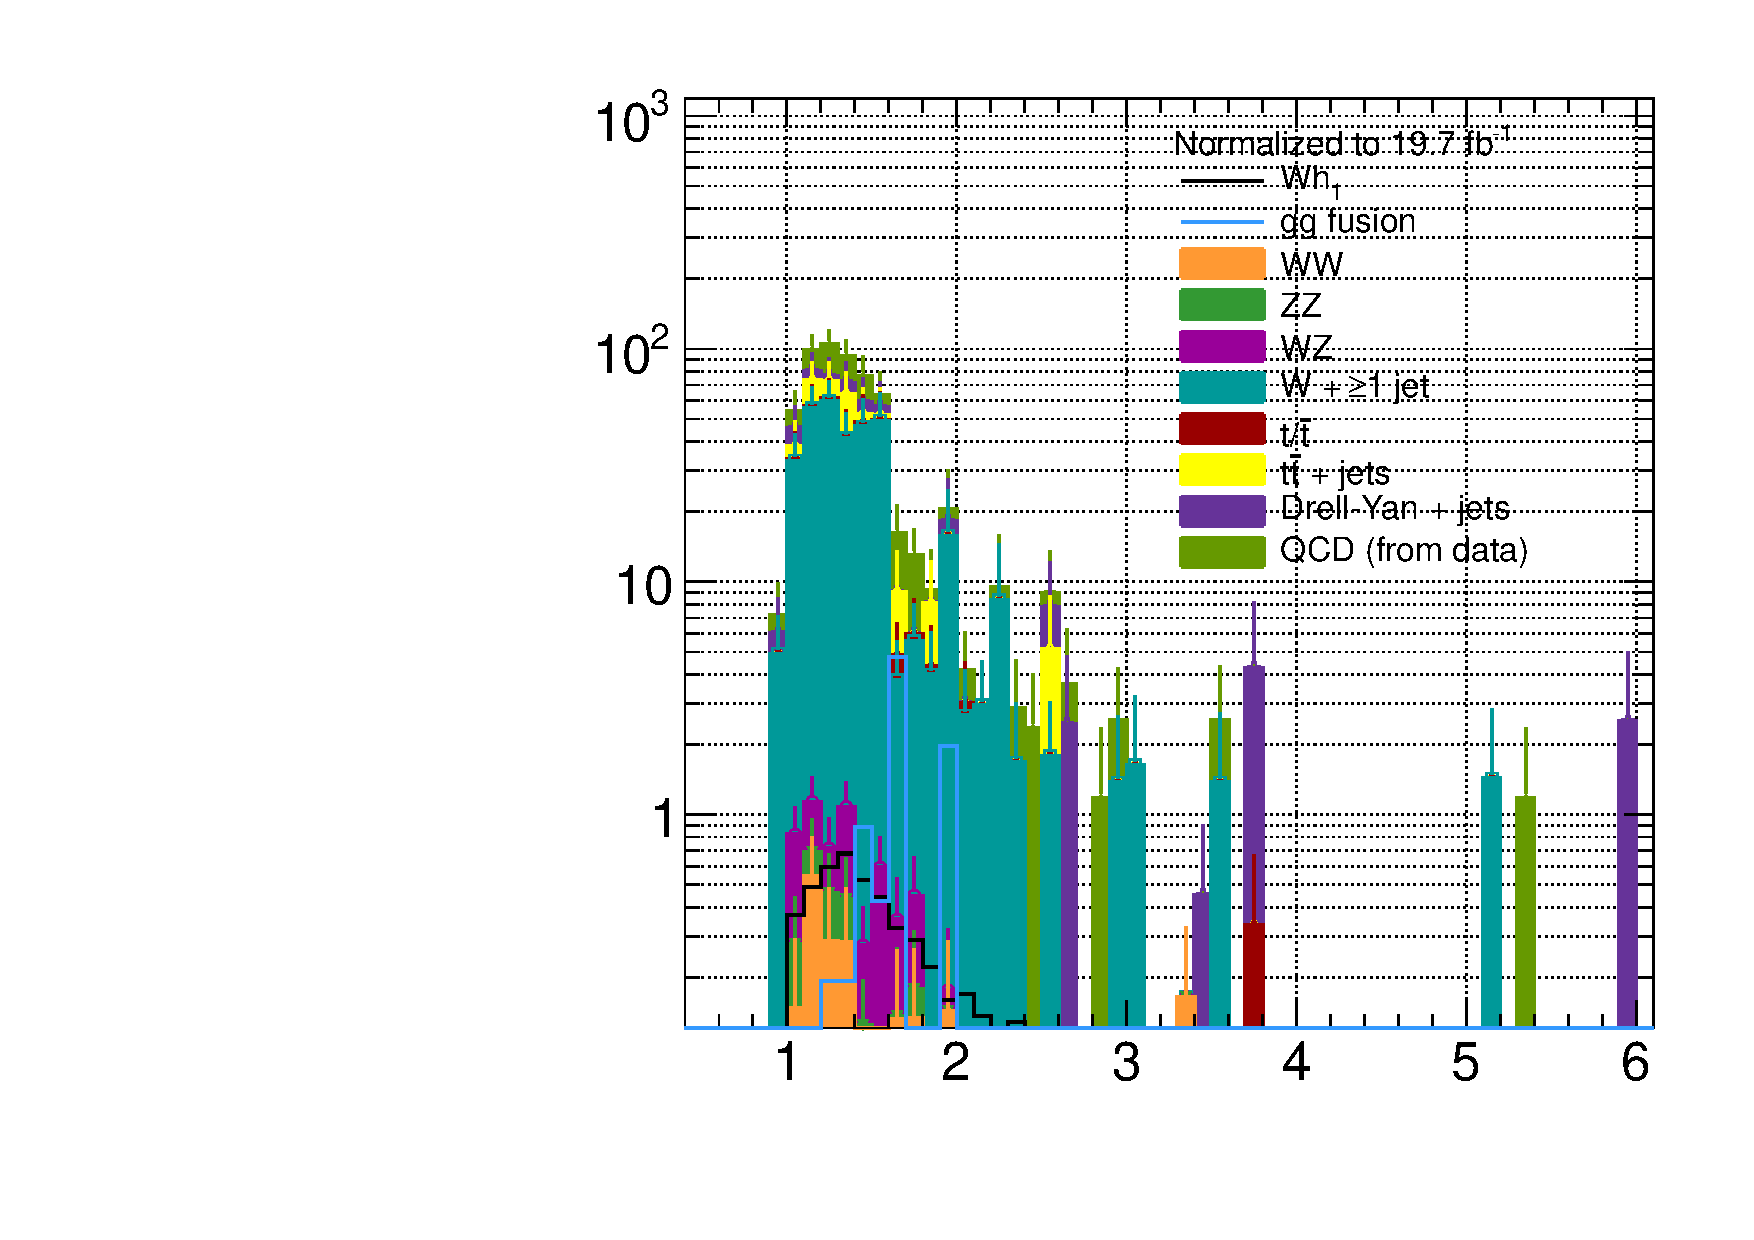
\includegraphics[width=1.2\cmsFigWidth]{figures/sigVsBkg_t1t2_highMT}
    \caption{Examples of N-subjettiness ratio distributions for the high-$M_{T}$ bin, comparing distributions for two signal models and all backgrounds discussed in Sec.~\ref{sec:evtsel} including data-driven QCD, after all the preselection cuts have been applied. (\cmsLeft) $\tau_{3}/\tau_{1}$. (\cmsRight) $\tau_{1}/\tau_{2}$.}
    \label{fig:nsubjettiness-ratios-highMT}
  \end{center}
\end{figure}
